\documentclass[12pt,a4paper]{article}

\usepackage{mystyle}

%\loadglsentries[main]{tex/glossar}
%\makeglossaries%Glossar
%\makeindex
\begin{document}
\begin{titlepage}
\begin{center}

% Oberer Teil der Titelseite:

\includegraphics[width=0.80\textwidth]{img/oc-logo.jpg}\\[1cm]

\textsc{\LARGE Dokumentation des AI Projektes}\\[1.5cm]

\textsc{\Large Allgemeine Informatik flexibel}\\[0.5cm]
\textsc{\Large Fachhochschule Köln}\\[0.5cm]

% Title
\newcommand{\HRule}{\rule{\linewidth}{0.5mm}}
\HRule \\[0.4cm]
{ \huge \bfseries Gegenüberstellung zweier Frameworks in Bezug auf deren Tauglichkeit zur Entwicklung einer Bürgschaftsverwaltung}\\[0.4cm]
\HRule \\[1.5cm]

% Author and supervisor
\begin{minipage}{0.3\textwidth}
\begin{flushleft} \large
\emph{Author:}\\
\textsc{Mara Braun}
\end{flushleft}
\end{minipage}
\hfill
\begin{minipage}{0.6\textwidth}
\begin{flushright} \large
\emph{Unternehmen:} \\
\textsc{OPITZ CONSULTING Deutschland GmbH
Kirchstraße 6\\
51647 Gummersbach\\
www.opitz-consulting.com}
\end{flushright}
\end{minipage}

\vfill
% Unterer Teil der Seite
%{\large \today}
\end{center}
\end{titlepage}

\clearpage
%\input{./signature.tex}
\pagenumbering{roman}
\section*{Abstract}
Die OPITZ CONSULTING Deutschland GmbH ist seit einigen Jahren mit der Wartung einer Webanwendung zur Verwaltung von Bürgschaften betraut. Da diese Anwendung jedoch schon vor einigen Jahren entwickelt wurde, entspricht ihre Performanz nicht mehr den Anforderungen der heutigen Zeit. Daher soll die Anwendung neu entwickelt werden. Hierfür kommen zwei große Frameworks in Frage. Das erste Framework ist das Application Development Framework von Oracle, in dessen veralteter Version  die zugrunde liegende Anwendung ursprünglich erstellt wurde. Das zweite Framework ist das zur Zeit verbreitete Open Source Framework Grails.

Im folgenden Dokument sollen nun die beiden Frameworks miteinander verglichen werden. Dieser Vergleich soll die Vor- und Nachteile der beiden Frameworks gegenüberstellen, um zu evaluieren, welches sich besser zur Neuentwicklung der Bürgschaftsverwaltung eignet.
\tableofcontents
\listoffigures
%\listoftables
\clearpage
\pagenumbering{arabic}
\section{Einleitung}
Im Zeitalter des Internets sind Web Anwendungen und mit ihnen Web Application Frameworks immer beliebter geworden, weshalb es in der heutigen Zeit eine Vielzahl von Web Application Frameworks gibt. Dies erschwert die Auswahl eines geeigneten Frameworks für das eigene Projekt, was auch allgemein ein relavantes Thema in Softwarehäusern, wie z.B. der OPITZ CONSULTING Deutschland GmbH ist. Die OPITZ CONSULTING Deutschland GmbH ist seit einigen Jahren mit der Wartung der unterschiedlichsten Anwendungen betraut und erhält ebenfalls regelmäßig Aufträge zur Entwicklung neuer Software. Zu den zu wartenden Anwendungen gehört unter anderem die Web Anwendung "`AvaleNet"' eines Bankhauses, die in einer veralteten Version des Frameworks Application Development Framework (ADF) entwickelt wurde und nun neu entwickelt werden soll, da die Performanz der Anwendungen nicht mehr den Anforderungen der heutigen Zeit genügt. Hierzu muss eine Entscheidung getroffen werden, welches Framework zur Migration der Anwendung verwendet werden soll. Die Entscheidungsfindung, welches der beiden zur Auswahl gestellten Frameworks verwendet werden soll, ist Bestandteil des folgenden Dokumentes. Hierfür werden zunächst die fachlichen Details der beiden Frameworks erläutert (Kapitel \ref{cha:kapitel-2}), um im darauf folgenden Kapitel (Kapitel \ref{cha:kapitel-3}) die Vor- und Nachteile der Beiden besser nachvollziehen zu können. Diese Vor- und Nachteile, die mit Hilfe einer zur Vergleichbarkeit entwickelten Metrik ermittelt wurden (Kapitel \ref{sec:anforderungskatalog}), werden dann in Bezug zu der zu entwickelnden Anwendung "`AvaleNet"' gesetzt und gegenübergestellt (Kapitel \ref{cha:kapitel-4}). Zuletzt wird eine Gewichtung der einzelnen Kriterien vorgenommen (Kapitel \ref{sec:gewichtung}), anhand derer letztendlich entschieden wird, welches Framework sich am besten zur Migration der Anwendung eignet (Kapitel \ref{cha:fazit}).
\section{Theoretische Grundlagen}
\label{cha:kapitel-2}
Dieses Kapitel soll für ein grundlegendes Verständnis der Architektur von ADF und Grails und des Umfangs dieser Frameworks sorgen, um im nachfolgenden Vergleich (Kapitel \ref{cha:kapitel-3} und \ref{cha:kapitel-4}) der beiden die Vor- und Nachteile nachvollziehen zu können. Hierbei wird zunächst allgemein die Entstehung der Frameworks und die den beiden Frameworks zugrunde liegende MVC-Architektur (Kapitel \ref{sec:entstehung} und \ref{sec:mvc}) erläutert und nachfolgend auf die spezifische Architektur und die jeweiligen Eigenschaften der beiden Frameworks eingegangen (Kapitel \ref{sec:adf} und \ref{sec:grails}).

\subsection{Entstehung}
\label{sec:entstehung}
Mit der Einführung von SOA (Service Oriented Architecture) in der Softwareentwicklung hat die Entwicklung von traditionellen Webanwendungen, in denen die Anwendung eine vollständige Lösung ist, ein Ende gefunden. Moderne Anwendungen sind heute nicht mehr eine vollständige Lösung, sondern sie sind komponentenbasierte Benutzerschnittstellen, die lokale und remote Services für ihre Business Logik verwenden. \autocite[S. XXI]{OFDG2010}
\subsection{MVC Architektur allgemein}
\label{sec:mvc}
Die Model View Controller (MVC) Architektur wurde in den 1970er Jahren von Trygve Reenskaug für die Plattform Smalltalk entwickelt und spielt bis heute eine bedeutende Rolle in den meisten UI-Frameworks und dem UI-Design\autocite[S. 330]{PEAA2002}.
Wie der Name schon vermuten lässt, besteht die MVC Architektur aus drei Rollen, dem Model, dem View und dem Controller.
\begin{itemize}
\item Das Model ist ein nicht sichtbares Objekt, dass einige Informationen der Domäne, wie z.B. alle Daten und Verhalten enthält. Diese Daten und Informationen müssen nicht denen die in der UI verwendet werden entsprechen\autocite[S. 330]{PEAA2002}.

\item Die View dient dazu Informationen aus dem Model anzeigen zu können. Dies kann z.B. in Form einer HTML-Seite geschehen, in der die gewünschten Informationen des Models dann angezeigt werden\autocite[S. 330]{PEAA2002}.

\item Die letzte Rolle ist die des Controllers. Der Controller dient dazu Benutzereingaben anzunehmen, das Model zu manipulieren und das View Objekt zu aktualisieren\autocite[S. 330f]{PEAA2002}.
\end{itemize}
Die wichtigste Trennung ist die Trennung von Model und View. Der Grundgedanke hierbei ist, dass ein Entwickler, wenn er eine View (Ansicht) entwickelt, über andere Dinge nachdenkt, als wenn er das Model entwickelt. Beispielsweise denkt er bei der Entwicklung der View mehr über die Mechanismen der UI und bei der Entwicklung des Models mehr über die Geschäftsstrategie nach. Zudem möchte ein User eventuell ein und dieselbe Information aus dem Model in einer Anwendung auf unterschiedliche Weise dargestellt haben, was sich durch die Trennung von View und Model vereinfacht, da für jede Ansicht das selbe Model verwendet werden kann und sich nur die View ändert. Ein letzter Aspekt, der für die Trennung von Model und View spricht, ist dass nicht sichtbare Objekte meist besser zu testen sind als sichtbare und so durch die MVC-Architektur die Modellogik getrennt von der Benutzeroberfläche (GUI) getestet werden kann.
\begin{figure}[h]
\centering
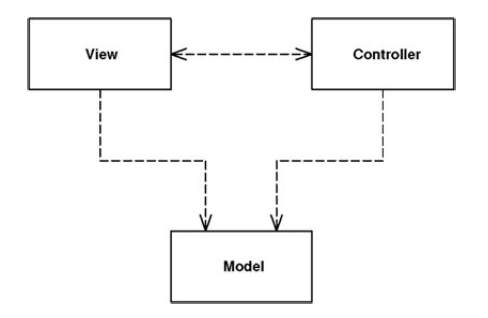
\includegraphics[width=0.80\textwidth]{img/MVC-Allgemein(Fowler).png}
\caption {MVC-Architektur \autocite[S. 330]{PEAA2002}}
\label{fig:mvc}
\end{figure}
Die Trennung von View und Controller dagegen ist weniger relevant und nicht immer sinnvoll, weshalb in einigen Frameworks heute eine Kombination von View und Controller verwendet wird. Selbst in den meisten Versionen von Smalltalk, für die die MVC-Architektur ursprünglich entwickelt wurde, wirde meist eine Kombination von View und Controller verwendet. Die Trennung von View und Controller ist vor allem dann sinnvoll, wenn es sich um Rich-Client-Systeme handelt oder der Controller von Web-Frontends separiert wird. \autocite[S. 330-332]{PEAA2002}\\
Wie auch in der Abbildung \ref{fig:mvc} zu sehen ist, ist die Richtung der Abhängigkeiten für die MVC-Architektur entscheidend. Die Abbildung zeigt, dass sowohl View als auch Controller vom Model abhängig sind, jedoch keine Abhängigkeit des Models von View oder Controller besteht. Diese Unabhängigkeit des Models bedeutet, dass das Model auch bei Änderungen an View und Controller unverändert bleibt und damit Änderungen am View deutlich erleichtert. \autocite[S. 330-332]{PEAA2002}
\subsection{ADF}
\label{sec:adf}
\subsubsection{Grundlegendes}
Eine Lösung zur Entwicklung von modernen Anwendungen als komponentenbasierte Benutzerschnittstelle bietet ORACLE mit dem Application Development Framework (ADF). ADF ist ein Java EE (Java Enterprise Edition) Framework, das Anwendungsentwicklung mit Java, Java EE und SOA vereinfachen soll um ein breites Publikum von Geschäftsbereich- und Technologieexperten anzusprechen, die zusammen arbeiten müssen, um langlebige Enterprise Softwarelösungen entwickeln zu können\autocite[S. XXIII]{OFDG2010}.
\subsubsection{Architektur}
Das Application Development Framework von Oracle basiert, wie auch einige andere Web Application Frameworks heutzutage auf der im vorigen Kapitel beschriebenen MVC-Architektur. 
Auch ADF hat Model, View und Controller, jedoch werden diese Schichten der Architektur noch durch die Ebenen Business Services und Data Services erweitert.
\begin{figure}[H]
\centering
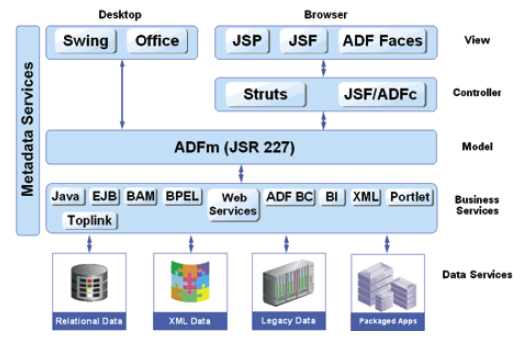
\includegraphics[width=0.80\textwidth]{img/MVC-ADF3.png}
\caption {MVC-Architektur von ADF \autocite[S.22]{AUW2009}}
\label{fig:mvc-adf}
\end{figure}

Die View Ebene der ADF Architektur (siehe Abbildung \ref{fig:mvc-adf}) ist, wie allgemein von der MVC Architektur vorgesehen, die Anzeigeebene der Anwendung und unterteilt sich in die Kategorien Desktop und Browser, da mit ADF sowohl Java Swing Anwendungen (also Desktopanwendungen) als auch Web- oder auch Browser-Anwendungen erstellt werden können \autocite[S.22]{AUW2009}. Diese Unterteilung wirkt sich auch auf die nächste Ebene der Architektur aus, denn eine Trennung von View und Controller wird für Desktopanwendungen nicht zwingend benötigt (siehe auch Kapitel \ref{sec:mvc}). Für Webanwendungen ist es jedoch sinnvoll einen Controller zu haben, um Frontend und Controller getrennt zu behandeln. Der Controller von ADF Anwendungen hat die Aufgabe, Benutzeraktionen zu interpretieren und zu entscheiden, welche Seiten dem User in welcher Reihenfolge angezeigt werden\autocite[S.12]{OAEAD2014}.\\
Das Model ist hier die Abstraktionsschicht. Es besteht aus dem ADF Binding Layer und den Data Controls. Die Data Controls bilden die Schnittstelle zu den Business Services und können daher verschiedene Geschäftslogikimplementierungen zur Verfügung stellen. Der Binding Layer verwendet wiederum die jeweilige vom Data Control zur Verfügung gestellte Geschäftslogik, um mit dem Controller (wenn er vorhanden ist) interagieren zu können und entsprechende Daten im View anzeigen zu können. \autocite[S.6]{ARIA2015}\\
Die beiden zusätzlichen Ebenen in der ADF-MVC-Architektur sind die Business Services und die Data Services. Mit Hilfe dieser Ebenen können in der Anwendung z.B. Web Services angebunden werden und  Verbindungen zu relationalen Datenbanken oder anderen Data Services hergestellt werden \autocite[S.13]{OAEAD2014}. Dies zeigt recht eindeutig, dass es sich bei ADF um ein sehr umfangreiches, nicht modulares Framework handelt, da der Stack der möglichen verwendbaren Technologien von vornherein feststeht und sich auch nicht mehr durch Erweiterungen oder ähnliches verändern lässt.

\subsection{Grails}
\label{sec:grails}
\subsubsection{Grundlegendes}
Auch Grails ist ein Framework, mit dem Web-Anwendungen erstellt werden können. Grails wurde 2005 unter anderem im Zuge der Beliebtheit von auf dynamischen Sprachen basierenden Frameworks entwickelt, die von Ruby on Rails angeführt wurde. Grails basiert auf der 2003 entstandenen Programmiersprache Groovy, die wiederum auf Java basiert\autocite[S.XXV]{DGG2002}\autocite[S.3]{GGR2009}. Das wesentliche Ziel des Frameworks Grails wurde wie folgt beschrieben: \begin{quote}\small "`The goal of Grails is to create a platform with the essence of frameworks like Rails or Django or CakePHP, but one that embraces the mature environment of Java Enterprise Edition(Java EE) and its associated APIs."'\autocite[S.4]{DGG2002}\end{quote} Grails soll also die guten Eigenschaften der bereits bestehenden Frameworks und Java EE verbinden um eine neues mächtiges Framework zu schaffen.

\subsubsection{Architektur}
Auch Grails verwendet, wie ADF und einige weitere Web Frameworks, die MVC-Architektur \autocite[S.208]{GGR2009}. Allerdings hält sich Grails strenger an die im ersten Kapitel beschriebene MVC-Architektur. Es gibt Model, View und Controller die miteinander agieren, wobei der Controller im Fall von Grails nicht optional ist, sondern immer benötigt wird, um eine Interaktion zwischen Model und View zu ermöglichen\autocite[S.8]{DGG2002}.\\
\begin{figure}[H]
\centering
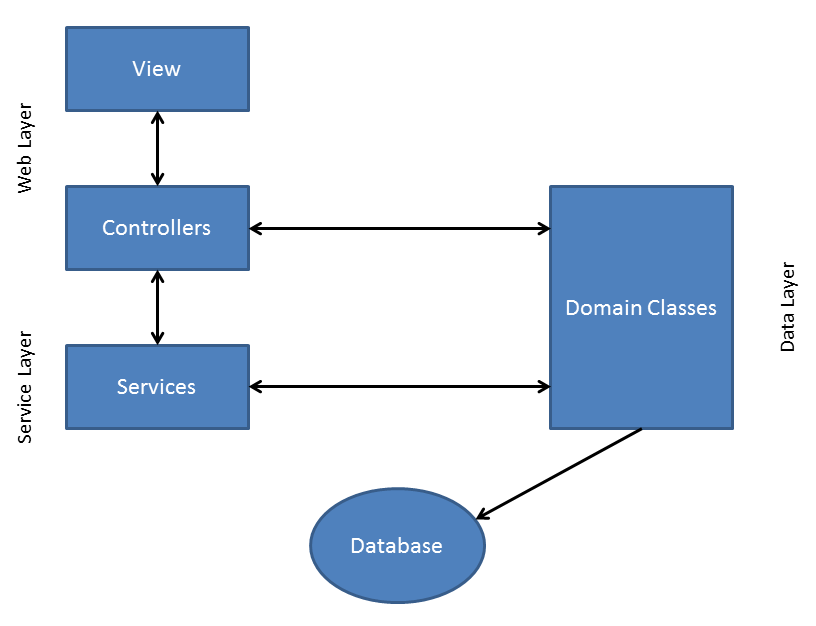
\includegraphics[width=0.80\textwidth]{img/Folie1.png}
\caption {MVC-Architektur von Grails \autocite[S.220]{GGR2009}}
\label{fig:mvc-grails}
\end{figure}
In Abbildung \ref{fig:mvc-grails} sowie auch im Framework selbst wird das Model durch Domain Klassen dargestellt. Diese Klassen sind persistent und werden von Grails automatisch einer jeweils zugehörigen physischen Tabelle in einer Datenbank zugeordnet \autocite[S.17]{DGG2002}. Diese Zuordnung kann zum Beispiel von der im Framework integrierbaren Technologie Hibernate übernommen werden \autocite[S.18]{DGG2002}. Grails lässt jedoch auch andere ORM (Object Relational Mapping) Systeme zu \autocite{GPO2015}. Des weiteren gibt es in Grails, wie auch in ADF die Möglichkeit, Services wie zum Beispiel RESTful Web Services anzubinden. Über die Abbildung (Abbildung \ref{fig:mvc-grails}) hinaus können zudem viele Funktionalitäten zusätzlich über Plugins hinzugefügt und verwendet werden \autocite[S.3]{DGG2002}.\\

In der folgenden Abbildung (Abbildung \ref{fig:tech-stack-grails}) wird der von Grails standardmäßig verwendete Technologiestack dargestellt. Es ist ersichtlich, dass Grails auf der Java Virtual Machine (JVM) aufbaut und Grails durch die verwendete Programmiersprache Groovy zudem die bekannte Java API und die entsprechenden zugehörigen Javadocs mit einem dynamischen Typsystem verbindet. Durch diese Verbindung ist sogar ein Mischen von statischen und dynamischen Typen möglich. \autocite[S.2-4]{DGG2002} 
\begin{figure}[h]
\centering
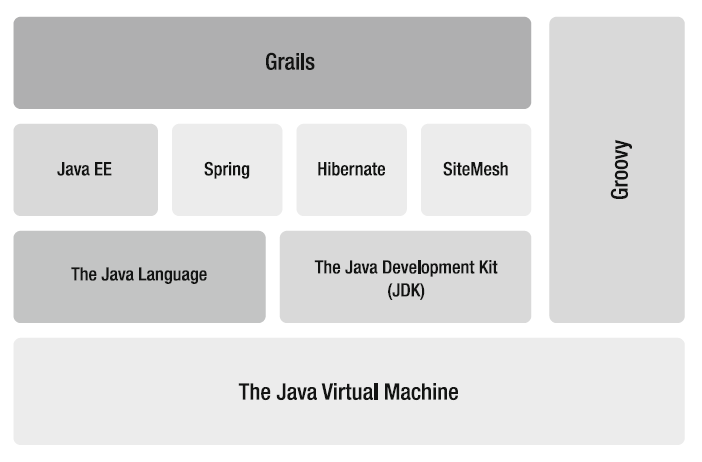
\includegraphics[width=0.80\textwidth]{img/Grails-Stack.png}
\caption {Technologiestack von Grails \autocite[S.3]{DGG2002}}
\label{fig:tech-stack-grails}
\end{figure} 
In Abbildung \ref{fig:tech-stack-grails} ist dies daran zu erkennen, dass sowohl Java als Sprache, als auch das Java Development Kit (JDK) Teil des Grails Technologiestacks sind. Allerdings sind die Komponenten Hibernate und Sitemesh und sogar die Programmiersprache Groovy optional, da statt Groovy auch Java verwendet werden kann und auch für Hibernate oder Sitemesh andere Komponenten verwendet werden können. Damit ist Grails ein sehr modulares Framework \autocite{GP2015}. Standardmäßig beinhaltet der Grails Technologiestack \autocite[S.2]{DGG2002}:
\begin{itemize}
\item Hibernate: Als Standard für objektrelationales Mapping (ORM)
\item Spring: das große und beliebte Open Source Inversion of Control Kontainer und Wrapper Framework für Java
\item SiteMesh: ein robustes und stabiles Layout Rendering Framework
\item Jetty: ein embeddable Servlet Container
\item HSQLDB: Ein reines Java relationales Datenbank Management System (RDBMS) 
\end{itemize}
\section{Gegenüberstellung der Frameworks}
Dieses Kapitel soll die wesentlichen Anforderungen an Web Application Frameworks ausführen und eine Begründung enthalten, weshalb diese Anforderungen relavant sind. Es wird benötigt, um in den folgenden Kapiteln die Vor- und Nachteile der beiden Frameworks vergleichbar darstellen zu können.
\subsection{Anforderungen an Web Application Frameworks}
\subsubsection{Lizenz und Lizenzkosten}
Da es sowohl Open Source als auch lizenzierte Frameworks zur Entwicklung von Webanwendungen gibt, können sich die eventuell vorhandenen Lizenzkosten auf die Gesamtkosten des Projektes auswirken. Zudem müssen anfallende Lizenzkosten zum Betreiben der entwickelten Software bei der Auswahl eines Frameworks mit betrachtet werden.
Ein weiterer zu beachtender Punkt bezüglich der Lizenzen ist die GNU General Public License (GNU GPL), denn sobald Teile des Quellcodes einer Software die unter diese Lizenz fällt in der eigenen Anwendung verwendet werden kann die Notwendigkeit bestehen, dass die eigene Anwendung ebenfalls unter diese Lizenz fallen muss. Daher ist insbesondere bei der Verwendung von GNU GPL Erweiterungen zu prüfen ob die Anwendung bei Verwendung ebenfalls unter die GNU GPL fällt.\autocite[S.214]{EFCMW2013} 
\subsubsection{Entwicklungsgeschwindigkeit}
Die mögliche Geschwindigkeit mit der mit einem Framework entwickelt werden kann ist sehr entscheidend bei der Wahl des Frameworks, da die Entwicklungszeit und damit auch die Kosten für den Kunden möglichst gering gehalten werden sollen. Aus diesem Grund sollte auf diesen Aspekt geachtet werden. In die tatsächliche Entwicklungsdauer fließt jedoch auch noch die Lernkurve mit ein.\autocite[S.214]{EFCMW2013}
\subsubsection{Lernkurve}
Da Web Application Frameworks nicht alle gleich aufgebaut oder ähnlich umfangreich sind, kann auch die Einarbeitungszeit für das entsprechende Framework unterschiedlich lang ausfallen. Da dies die Entwicklungszeit für die entsprechende Software verlängern oder verkürzen kann, gilt es die Lernkurve bei Auswahl des Frameworks zu beachten.\autocite[S.214]{EFCMW2013}
\subsubsection{Community}
Für die Entwicklung mit einem entsprechenden Framework kann die vorhandene Community ein essentieller Bestandteil sein, denn immer wieder können bei der Entwicklung Fehler oder Probleme auftreten, deren Lösung viel Zeit in Anspruch nehmen kann. In einer großen Community kann das Problem aber bereits von einem anderen Entwickler gelöst und festgehalten worden sein oder aber es wird auf Anfrage von jemandem gelöst, was einiges an Zeit einsparen kann.
\subsubsection{Testbarkeit}
Die Testbarkeit von Software ist allgemein sehr wichtig, da Software zum einen komplex ist und sich zum anderen häufig ändern kann. Auf Grund dieser beiden Aspekte, ist es möglich, dass durch Änderungen Fehler entstehen können die in der komplexen Software vielleicht zunächst nicht auffallen. Eine gute Testabdeckung kann verhindern, dass solche Fehler übersehen werden.
\subsubsection{Umfang und Qualität der Dokumentation}
Eine umfangreiche und verständliche Dokumentation ist sehr wichtig um mit dem Framework arbeiten zu können. Eine schlechte Dokumentation führt schnell zu Verwirrung und Frustration und verlangsamt damit auch die Entwicklungsgeschwindigkeit. Eine umfangreiche und mit Beispielen versehene Dokumentation ist daher wichtig für die Auswahl des Frameworks.\autocite[S.214]{EFCMW2013}
\subsubsection{Modularität}
Da es sehr viele verschiedene Verwendungsmöglichkeiten für Web Anwendungen mit sehr unterschiedlichen Funktionsanforderungen gibt, ist es häufig sinnvoll nicht alle möglichen Funktionalitäten im Framework zu integrieren, sondern diese durch Erweiterungen (im nächsten Punkte näher erläutert) verfügbar zu machen. Ein leichtgewichtigeres Framework ist für kleine Webanwendungen daher besser geeignet, da weniger nicht benötigte Funktionen enthalten sind und die Komplexität des Frameworks nicht unnötig vergrößern.\autocite[S.214]{EFCMW2013}
\subsubsection{Erweiterbarkeit}
Bei der Entwicklung einer Web Anwendung ist es gut möglich, dass Funktionen verwendet werden sollen, die für sehr viele Web Anwendungen die selben sind (z.B. die Authentifizierung). Daher ist die Erweiterbarkeit des Frameworks und die Möglichkeit der Verwendung von Plugins für Web Application Frameworks ein wesentlicher Aspekt.\autocite[S.214]{EFCMW2013}
\subsubsection{Versionierbarkeit}
Da Software und damit auch Webanwendungen häufig im Team entwickelt werden, muss eine Möglichkeit zur Versionierung der zu entwickelnden Anwendung gegeben sein. Hierbei ist es wünschenswert, dass beim Zusammenführen der verschiedenen Entwicklungsstände möglichst wenig Konflikte auftreten. Weiterhin sollte gute Versionierung Änderungen im Nachhinein nachvollziehbar machen.
\subsubsection{Langlebigkeit}
Die Langlebigkeit eines Frameworks ist insbesondere im Bezug auf den zugehörigen Support und Sicherheitsupdates relevant, da diese mit dem Aussterben des Frameworks ebenfalls wegfallen. Es ist also für eine Anwendung die für eine lange Dauer zum Einsatz kommen soll zu beachten, dass auch das Framework für diese Dauer warscheinlich weiterhin unterstützt wird.\autocite[S.214]{EFCMW2013}
\subsubsection{Performanz}
Die Performanz von Web Application Frameworks und den daraus resultierenden Anwendungen ist ebenfalls ein wesentlicher Punkt bei der Auswahl eines Frameworks, jedoch wird dieser hier nicht genauer betrachtet, da es schwer ist sinnvoll vergleichbare Werte für die Performanz zweier Frameworks zu finden.
\subsection{Vor- und Nachteile von ADF}
Da ADF eine proprietäre kommerzielle Software ist fallen bei Einsatz der, mit diesem Framework entwickelten, Software Lizenzkosten an. Jedoch hat die Verwendung eines proprietären Frameworks den Vorteil, das der Quellcode in keinem Fall offen gelegt werden muss, wie es bei der GNU GPL\autocite{GNU2015} der Fall ist, was für einige Kunden essentiell ist. Der Aufbau des Frameworks ADF lässt jedoch nicht als modular bezeichnen, da ADF ein kaum erweiterbares Framework ist und entsprechend den gesamten Umfang der möglichen Funktionen schon zu Beginn enthält. Dieser große Umfang des Frameworks wirkt sich wiederum auf die Lernkurve des Frameworks aus und bewirkt, dass das Framework insbesondere für Entwickler mit wenig Erfahrung im Java Enterprise Umfeld schwerer zu erlernen ist\autocite[S.24]{AUW2009}. Einen Überblick über das Framework ADF zu bekommen kann daher einiges an Zeit erfordern und wirkt sich damit negativ auf die Entwicklungsdauer aus. Einem Entwickler, der bereits Erfahrung mit ADF gesammelt hat und mit ADF vertraut ist, ist das sogenannte "`Rapid Application Development"' möglich, das ADF durch seinen baukastenartigen Aufbau und die vielen Wizards ermöglicht \autocite[S.3]{ARIA2015}. Dieses schnelle Entwicklungstempo wird zudem durch die umfangreiche Dokumentation und den Support von Oracle selbst durch zahlreiche Tutorials für die unterschiedlichsten Problemszenarien unterstützt. Die zu ADF gehörige Community ist weltweit deutlich kleiner als die zum Framework Grails gehörige. Dies lässt sich anhand der folgenden Abbildung erkennen. 
\begin{figure}[h]
\centering
\includegraphics[width=\textwidth]{img/interesse_zeitl.png}
\caption{Zeitverlauf des Interesses an ADF und Grails weltweit \autocite{GT2015} }
\end{figure}
Die Grafik zeigt den zeitlichen Verlauf des Interesses an den beiden Frameworks ADF (in rot) und Grails (in blau) weltweit anhand der Häufigkeit\footnote{für genauere Erläuterung zur Wertefindung im Diagramm: http://goo.gl/Ma9kWJ} von Suchanfragen über Google. Das Suchinteresse wird hierbei relativ zum Höchstwert dargestellt. Diese Grafik lässt den Schluss zu, dass ADF zwar eine kleinere Community hat aber sich durchaus als langlebig erwiesen hat, da das Interesse an ADF mehr oder weniger konstant bleibt. Die Langlebigkeit des Frameworks, die auch in Zukunft zu erwarten ist bietet den Vorteil, dass auch der Support weiterhin besteht und damit auch spätere Wartungsaufgaben erfüllbar sind \autocite[S.214]{EFCMW2013}. Auch die im Anforderungskatalog aufgeführten Punkte Versionierbarkeit und Testbarkeit erfüllt ADF, da es sich zum einen mit den bekannten Versionierungstools GIT und SVN versionieren lässt und damit auch die Arbeit in größeren Teams zulässt, zum anderen aber auch beispielsweise Unit Tests möglich sind um z.B. selbst erstellte Java Klassen und Methoden testen zu können. Bei der Versionierbarkeit gilt es jedoch zu beachten, dass nicht jeder Schritt für andere Entwickler Nachvollziehbar bleibt, da ADF viele Wizards zur Erstellung von Funktionen, Klassen und Dateien bietet. Diese Wizards sind aus der Sicht von GIT und SVN die rein textbasiert arbeiten nicht immer nachvollziehbar.

\subsection{Vor- und Nachteile von Grails}
Grails ist ein modulares Open Source Framework, dass unter die Apache License in der Version 2.0 fällt. Diese Lizenz hat zunächst keine Auswirkungen auf die zu entwickelnde Anwendung, da im allgemeinen diese Lizenz nur eine Auswirkung hätte, wenn das Framework Teile des eigenen Source Codes in das Programm kopieren würde \autocite{AL2015}. Dies kann aber bei Grails höchstens bei Plugins (den zahlreichen Erweiterungsmöglichkeiten von Grails) vorkommen, die wiederum alle ihre eigenen Lizenzen haben. Dies hat wiederum den Nachteil, dass man für jede der vielen möglichen Erweiterungen des Frameworks, die man verwenden möchte zunächst überprüfen muss ob die Lizenz Auswirkungen auf die zu entwickelnde Software hat. Diese Überprüfungen können wenn sie notwendig sind, negative Auswirkungen auf die Entwicklungsgeschwindigkeit haben. Ansonsten sind Entwicklungsgeschwindigkeit und Lernkurve für Entwickler mit Java Vorkenntnissen sehr gut, da diese Grails schnell lernen können und entsprechend schnell entwickeln können. Grails bietet allerdings weniger Wizards und ist nicht wie ADF nach dem Baukasten Prinzip für "`Rapid Application Development"' ausgelegt. Es muss also der meiste Code selbst geschrieben werden. Durch sehr viel selbst geschriebenen Code wird sowohl eine umfangreiche Testabdeckung, als auch eine gute Dokumentation und Commmunity benötigt. Diese Punkte sind gegeben, da Grails die Java basierte Programmmiersprache Groovy verwendet und damit zum einen die gleichen Testmöglichkeiten bestehen, zum anderen aber auch die Javadocs als Dokumentation gültig sind, welche sehr umfangreich sind. Zusätzlich zu der Java Dokumentation hat Grails aber auch eine eigene umfangreiche Dokumentation und eine große Community, die in entsprechenden Foren Fragen beantwortet und Beispiele für verschiedene Problemstellungen zur Verfügung stellt. Wie auch für ADF lässt sich die Größe der Community etwa am Zeitverlauf des Interesses an den beiden Frameworks (siehe Abbildung 5: Zeitverlauf des Interesses an ADF und Grails weltweit
) und an den Einträgen in dem wohl meist genutzten Portal "`Stackoverflow"'\autocite{SOFG2015} ablesen. Was die Langlebigkeit von Grails betrifft so ist das Interesse an Grails weniger konstant, jedoch ist es hoch genug um davon ausgehen zu können, dass Grails noch einige Zeit bestehen wird. Ein Weiterer für Webapplication Frameworks relevanter Punkt ist die Versionierbarkeit. Das Versionieren der zu entwickelnden Software via z.B. SVN oder GIT ist problemlos möglich. Hierbei hat Grails jedoch den Vorteil, dass durch den vielen eigenen Code und weniger Wizards die ausgeführten Schritte später leichter nachzuvollziehen sind, was für Entwicklung in großen Teams ein großer Vorteil ist.
\section{Projektspezifische Gegenüberstellung}
\label{cha:kapitel-4}
Dieses Kapitel soll die zu erstellende Anwendung "`AvaleNet"' grundlegend beschreiben (Kapitel \ref{sec:hintergrund} und \ref{sec:anforderung}), um einen Einblick zu erhalten, welche Aspekte der beiden Frameworks ADF und Grails für die Anwendung relevant sein können. Zudem sollen die im vorigen Kapitel (Kapitel \ref{cha:kapitel-3}) erläuterten Vor- und Nachteile der beiden Frameworks Grails und ADF im Bezug auf die zu entwickelnde Anwendung verglichen und gewichtet werden (Kapitel \ref{sec:vergleich}),um letztendlich zu entscheiden, welches der beiden Frameworks sich besser zur Entwicklung der Anwendung "`AvaleNet"' eignet (Kapitel \ref{sec:gewichtung} und \ref{cha:fazit}).
\subsection{"`AvaleNet"'}
\subsubsection{Projekthintergrund}
\label{sec:hintergrund}
Die zu migrierende Anwendung "`AvaleNet"' ist die Web Anwendung eines Bankhauses zur Verwaltung von Bürgschaften. Dies beinhaltet unter anderem die Verwaltung von Kunden-, Konto- und Avaldaten. Die Anwendung "`AvaleNet"' wurde vor sechs Jahren in einer heute veralteten Version (Version 10) des Frameworks ADF entwickelt. Da dies eine heute schlechte Performanz der Anwendung und eine erschwerte Wartbarkeit zur Folge hat, soll die Anwendung nun migriert werden. Hierfür stehen die beiden Frameworks ADF und Grails zur Auswahl.
\subsubsection{Projektanforderungen}
\label{sec:anforderung}
Die Anwendung "`AvaleNet"' dient zur Verwaltung von Bürgschaften, hierbei müssen Kundendaten mit zugehörigen Konten sowie Daten zu den Bürgschaften selbst gespeichert werden. Diese Daten werden in einer relationalen Datenbank abgelegt, auf die die Anwendung "`AvaleNet"' sowohl lesend als auch schreibend zugreifen kann. Die Avale, sowie die Konten der Kunden sollen über Listen anzeigbar sein, wobei ein Wechsel zu einer Detailansicht eines Kontos oder eines Avals möglich ist. Außerdem ermöglicht es die Anwendung einem Mitarbeiter des Bankhauses, bereits bestehende Daten von Kunden, Konten oder Avalen zu bearbeiten und es stehen ihm einige Export-Funktionen zur Verfügung. Er kann beispielsweise eine Liste aller, zu einem Kunden gehörigen, Avale in ein PDF-Dokument exportieren, oder die Einzeldaten pro Aval auf diese Weise auflisten lassen. Zudem sollen alle Änderungen in der Anwendung historisiert werden, um auch über bereits getilgte Avale Bescheid zu wissen und nachhalten zu können, wer zuletzt welche Änderung vorgenommen hat.

\subsection{Vor- und Nachteile der Frameworks im Bezug auf "`AvaleNet"'}\label{sec:vergleich}
Der zunächst wichtigste Aspekt bei der Auswahl eines Web Applikation Frameworks ist, dass das entsprechende Framework alle Funktionalitäten enthalten muss, die für die Umsetzung des geplanten Projektes notwendig sind. Dabei müssen die Funktionalitäten nicht von vornherein im Grundumfang des Frameworks vorhanden sein, sondern sie können auch durch Erweiterungen des Frameworks später hinzuzufügen sein. \\\\
Für "`AvaleNet"' erfüllen beide Frameworks diesen Anspruch, da die Anwendung mit ihren Funktionen nur wenig über die Standard Funktionen einer Web Anwendung hinausgeht. ADF beinhaltet diese Funktionen schon im Grundumfang des Frameworks und für Grails lassen sich die zusätzlich benötigten Funktionen über Erweiterungen (Plugins) hinzufügen. \begin{table}[h]
  \centering
    \begin{tabular}{l l}
	  \toprule
	  Verwendetes Plugin & Lizenz \\
	  \midrule
	  Spring Security Core Plugin &  Apache License 2.0 \\
	  Hibernate Grails Plugin &  Apache License 2.0  \\
	  Jquery Grails Plugin &  Apache License 2.0  \\
	  Rendering Grails Plugin &  Apache License 2.0  \\
	  Tomcat Grails Plugin &  Apache License 2.0  \\
	  \bottomrule
    \end{tabular}
    \caption{Verwendete Plugins und zugehörige Lizenzen \autocite{GP2015}}
    \label{tab:plugins}
  \end{table}Zudem hat ADF bezüglich der zu entwickelnden Anwendung "`AvaleNet"' den Vorteil, dass es sich um ein proprietäres Framework handelt und damit keinesfalls der Quellcode der Anwendung offengelegt werden muss. Dies ist gerade bei einer Anwendung für ein Bankhaus relevant, die mit sensiblen Kundendaten agiert. Allerdings ist auch die Verwendung von Grails hier nicht kritisch, da kaum zusätzliche Plugins verwendet werden und diese keine kritischen Lizenzen enthalten (siehe Tabelle \ref{tab:plugins}), die den Entwickler zwingen, die zu entwickelnde Software ebenfalls zu einer Open Source Software zu machen. Einzig das Rendering Plugin, das selbst auch unter die Apache Lizense 2.0 fällt verwendet Bibilotheken, die unter die GNU Lesser General Public License\autocite{LGPL2015} (LGPL) fallen. Diese beinhaltet ebenfalls kein starkes Copyleft und zwingt den Nutzer so ebenfalls nicht den Quellcode offen zu legen.\\\\
  Der Grund für die geringe Notwendigkeit von Plugins ist, dass "`AvaleNet"' eine kleine Anwendung ist, die keine umfangreiche Funktionalität erfordert. Dies hat ebenfalls zur Folge, dass die Entwicklung der neuen Anwendung kein großes Team erfordert, sondern von einer Person mit geringem Zeitaufwand (weniger als ein halbes Jahr) umgesetzt werden kann. Da die mit der Entwicklung betraute Person zudem hauptsächlich Kenntnisse im Java Umfeld und keine Erfahrung mit ADF hat spielt die Lernkurve hier für die gesamte Entwicklungsdauer inklusive Einarbeitungszeit eine große Rolle. So hat Grails den Vorteil, dass es mit Java Grundkenntnissen schneller zu erlernen ist als ADF ohne Vorkenntnisse. Ein weiterer Nachteil von ADF bezüglich "`AvaleNet"' ist, nicht vorhandene Modularität und der damit verbundene Überfluss an Funktionen, die das Framework bereitstellt, welche aber für eine solch kleine Anwendung nicht benötigt werden. Zudem erschweren sie es dem Entwickler, das Framework schneller zu erlernen. \\\\
  Unabhängig von dem im vorigen Kapitel aufgestellten Anforderungskatalog hat ADF jedoch den Vorteil, dass die zu migrierende Anwendung bereits in ADF geschrieben wurde und ein erfahrener Entwickler die Anwendung daher mithilfe der alten Anwendung deutlich schneller in der neuen Version von ADF (12.0.3) nachbauen könnte. Zudem ist ein Großteil der benötigten Lizenzen für die Verwendung einer ADF Anwendung zusammen mit einer Oracle Datenbank bereits vorhanden und es würden bei Verwendung der neuen Version von ADF damit keine großen Mehrkosten anfallen. Allerdings gibt es in dem mit der Wartung und Migration betrauten Unternehmen (OPITZ CONSULTING Deutschland GmbH) nur wenige Mitarbeiter mit umfangreichen ADF Kenntnissen, dafür aber einige mit guten Java- und Grailskenntnissen, weshalb Grails für diese Situation von Vorteil wäre. \\\\
  Diese Verteilung des Interesses ist nicht unüblich, wie die Grafik zum Interesse an ADF und Grails weltweit bereits gezeigt hat. Auch für Deutschland zeigt diese Verteilung, dass das Interesse an ADF deutlich geringer ist als das an Grails (Abbildung \ref{fig:gtd15}). Dieses stärkere Interesse an dem Framework Grails hat den Vorteil, dass in einem Forum, wie dem viel genutzten Forum "`Stackoverflow"' deutlich mehr Einträge zu Grails zu finden sind als zu ADF. Grails ist dort mit 21260\autocite{SOFG2015} beantworteten Fragen vertreten und ADF mit nur 1031\autocite{SOFA2015}.

\begin{figure}
\centering
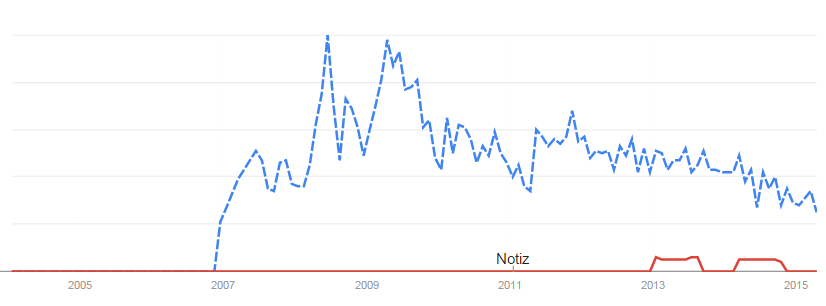
\includegraphics[width=\textwidth]{img/interesse_de.png}
\caption{Zeitverlauf des Interesses an ADF und Grails in Deutschland \autocite{GT2015}}
\label{fig:gtd15}
\end{figure}

\subsection{Aufwiegen der Vor- und Nachteile}
\label{sec:gewichtung}
Von den in den vorigen Kapiteln aufgeführten Kriterien zur Auswahl eines Web Application Frameworks sind insbesondere die Kriterien Lizenz und Lizenzkosten, Entwicklungsgeschwindigkeit, Lernkurve, Umfang und Qualität der Dokumentation und Modularität von großer Bedeutung für die Anwendung "`AvaleNet"'. Zu begründen ist dies damit, dass diese Kriterien insbesondere die Kosten für das Projekt und den Arbeitsaufwand gering halten, denn ein modulares Framework verkürzt die Einarbeitungszeit und damit die Entwicklungsdauer. Dies wird ebenfalls durch eine gute Dokumentation gestützt. Hier bietet Grails im Gegensatz zu ADF den Vorteil, dass es keine Lizenzkosten  hat. Lizenzkosten fallen hierbei nur bei der Verwendung einer Oracle Datenbank an, welche aber bereits besteht. Aus diesem Grund bedeuten diese Lizenzkosten keine Mehrkosten für den Kunden. Zudem ist die Lernkurve von Grails deutlich besser als die von ADF, da Grails deutlich modularer aufgebaut ist. Die Entwicklungsgeschwindigkeit ist der einzige Punkt in dieser Auflistung, in dem ADF besser geeignet ist als Grails, da ADF das sogenannte "`Rapid Application Development"' ermöglicht. Jedoch steht die geförderte Entwicklungsgeschwindigkeit in keinem Verhältnis zur benötigten Einarbeitungszeit, weshalb dies für ein so kurzes Projekt kaum eine spürbare Auswirkung hätte. Für größere Projekte kann die gesteigerte Entwicklungsgeschwindigkeit allerdings durchaus ein Grund sein, ADF Grails vorzuziehen. \\

Weniger wichtig, aber ebenfalls von Bedeutung sind die Kriterien Community, Testbarkeit, Erweiterbarkeit und Fähigkeiten im Unternehmen, weil sie ein möglichst reibungsfreies Entwickeln ermöglichen und sicherstellen, dass die Anwendung später möglichst fehlerfrei funktionieren kann. Auch hier bietet Grails mehr Vorteile als ADF, da Grails zum einen eine deutlich größere Community und damit schnellere Hilfe bei auftretenden Problemen bietet und zum anderen eine große Anzahl an Erweiterungen zur Verfügung stellt und es ermöglicht eigene Erweiterungen zu schreiben. Diese Anzahl möglicher Erweiterungen kann jedoch für andere Projekte, die weniger Standard Plugins verwenden, zum Nachteil werden, da es Zeit kostet, die richtige Erweiterung mit einer zu den Anforderungen des Projektes passenden Lizenz zu finden. Auerdem lässt es sich teilweise nicht von vornherein sagen, ob sich ein Plugin tatsächlich für ein Vorhaben eignet.\\

Für "`AvaleNet"' eher unwichtig sind Versionierbarkeit und Langlebigkeit, da für eine einzelne Person Versionierung zwar sinnvoll ist, um immer einen lauffähigen Stand der Anwendung zu haben und diesen widerherstellen zu können. Dies lässt sich jedoch auch über regelmäßige Sicherungen des Projektes realisieren und erfordert nicht zwingend ein Versionierungstool. Die Langlebigkeit des Frameworks wird hier als weniger wichtig eingestuft, da das Framework primär zur Entwicklung der Anwendung bewertet wird und eine weitere Unterstützung des Frameworks hauptsächlich Auswirkungen auf den späteren Support bei Wartung der Anwendung hat. Im Bezug auf die Langlebigkeit hat das proprietäre Framework ADF allerdings den klaren Vorteil, dass ein Framework, dass Lizenzkosten erfordert, auch für eine gewisse Dauer den Support und das Bestehen des Frameworks und der zugehörigen Komponenten garantiert, wohingegen das Bestehen von Grails sehr stark von der Popularität des Frameworks und der Aktivität der Community abhängt.
  \begin{table}[H]
  \centering
    \begin{tabular}{l l l l}
	  \toprule
	  Relevanz & Kriterien & ADF & Grails \\
	  \midrule
	  hoch & Lizenzkosten & schlecht & gut \\
	  & Lizenz & gut & gut \\
	  & Entwicklungsgeschwindigkeit & sehr gut & gut \\
	  & Lernkurve & schlecht & gut\\
	  & Dokumentation & gut & gut \\
	  & Modularität & schlecht & sehr gut \\
	  \midrule
	  mittel & Community & gut & sehr gut \\
	  & Testbarkeit & gut & gut \\
	  & Erweiterbarkeit & schlecht & gut \\
	  & Skill im Unternehmen & schlecht & gut \\
	  \midrule
	  niedrig & Versionierbarkeit &  gut & sehr gut \\
	  & Langlebigkeit &  sehr gut & gut \\
	  \bottomrule
    \end{tabular}
    \caption{Übersicht über Entscheidungskriterien}
  \end{table}
\section{Fazit}
Dieses Kapitel fasst noch einmal zusammen, weshalb das Framework Grails gewählt wurde und welches nach der Gegenüberstellung besser zur Entwicklung geeignet ist.\\\\
Zur Migration der Web Anwendung "`AvaleNet"' in eine neue Version eignet sich im Gegensatz zu dem proprietären Application Development Framework (ADF) von Oracle das Open Source Web Application Framework Grails am besten. Dies ist damit zu Begründen, dass unter Anderem für eine Grails Anwendung im Gegensatz zu einer ADF Anwendung keine zusätzlichen Lizenzkosten anfallen. Des weiteren ist Grails ein modulares Framework, das sich nahezu beliebig erweitern lässt. Dies bietet gegenüber ADF den Vorteil, dass sich der Entwickler nur mit den benötigten Funktionen des Frameworks auseinandersetzen muss und es damit deutlich schneller erlernen kann.
Bezogen auf die Ausgangssituation, dass die neue Anwendung von einem noch unerfahrenen Entwickler mit Java Vorkenntnissen entwickelt werden soll, wirkt sich die Verwendung von Grails zudem positiv auf die Entwicklungsgeschwindigkeit und -Dauer aus.
\clearpage
\addcontentsline{toc}{section}{Literaturverzeichnis}
%\bibliographystyle{plain}
\bibliography{literatur}
%\printglossary[title=Glossar]%Glossar ausgeben
\clearpage
%\input{tex/anhang}
\end{document}

%%% Local Variables:
%%% mode: latex
%%% TeX-master: t
%%% End:
